\subsubsection{On-Demand Replica Generation for a New Pattern}
\label{sec:rep_generate}
%
\begin{algorithm} [tb!]
 \caption{\textsc{Build Replica for a New Pattern}}
 \label{algo:getreplica}
{\scriptsize
 \dontprintsemicolon
 \nonl \textbf{Input:} data graph $G=(V,E,L)$, parent
 pattern $Q=(V_Q,E_Q,$ $L)$, $\mathcal{R}$eplica$(Q)=(V_{\mathcal{R}(Q)}$,
 $E_{\mathcal{R}(Q)}$, $L)$, child pattern $R=(V_R$, $E_R$, $L)$, extending node:
 $u\in V_Q$, extending edge: $(u,v) \in E_R$ \;
\nonl \textbf{Output:} $\mathcal{R}$eplica$(R)$ \;
	\vspace{0.3mm}
	$DFS\ List(Q)\leftarrow$ get edge list via rooted DFS in $Q$ with $u$ as root \;
	Initialize $instance \leftarrow \emptyset, $ $ \mathbb{I} \leftarrow \emptyset$\;
	\ForEach{ $u' \in Mapping(u,\ \mathcal{R}$\textup{eplica}$(Q))$}
	{
		$instance.{\sf add}(u\mapsto u')$\;
		\ForEach{\textup{edge} $(u',v')\in E_G$ \textup{that maps to the extending edge} $(u,v)\in E_R$}
		{
			$instance.{\sf add}(v\mapsto v')$\;
	        $\mathbb{I}\leftarrow$ \textsc{FindAllInstances($G$, $Q$, $\mathcal{R}eplica(Q)$, $R$,
	        $DFS\ List(Q)$, $instance$, $\mathbb{I}$)}\;
			\textsc{UpdateReplica($R$, $\mathcal{R}eplica(R)$, $\mathbb{I}$)}\;
			% $instance\leftarrow instance \setminus \{(v,v')\}$\;
			$instance.{\sf delete}(v\mapsto v')$\;
		}
		% $instance\leftarrow instance \setminus \{(u,u')\}$\;
		$instance.{\sf delete}(u\mapsto u')$\;
	}	
	\Return{$\mathcal{R}$\textup{eplica}$(R)$}\;}
\end{algorithm}
%
\vspace{-2mm}
\begin{algorithm}[tb!]
 \caption{\textsc{FindAllInstances:Exact Method}}
 \label{algo:findallinstances}
{\scriptsize
 \dontprintsemicolon
 \nonl \textbf{Input:} data graph $G=(V,E,L)$, parent
 pattern $Q=(V_Q,E_Q,$ $L)$, $\mathcal{R}$eplica$(Q)=(V_{\mathcal{R}(Q)}$,
 $E_{\mathcal{R}(Q)}$, $L)$, child pattern $R=(V_R$, $E_R$, $L)$,
    $DFS\ List(Q)$, partial isomorphism of $R$: $instance$, $\mathbb{I}$\;
\nonl \textbf{Output:} $\mathbb{I}: $ set of all instances of $R$ in $G$ consistent with input partial isomorphism $instance$\;
	\uIf{$instance$ \textup{is} {\sf Found}}
	{
		\Return{$\{instance\}$}
	}
	\Else
	{
		$e=(p,c)\leftarrow$ \textsc{NextQueryEdge($DFS\ List(Q)$)}\;
		$v' \leftarrow instance(p)$\;
		\uIf{$e$ \textup{is a} {\sf backward edge}}
		{
			\uIf{\textup{an edge} $(v',instance(c))$ \textup{exists in} $E_{\mathcal{R}(Q)}$}
			{
				$\mathbb{I} \leftarrow \mathbb{I}\ \cup$ \textsc{FindAllInstances({$G$}, $Q$, $\mathcal{R}eplica(Q)$, $R$, $DFS\ List(Q)$, $instance$, $\mathbb{I}$)}\;
			}
			\Else{\Return $\emptyset$}
		}
		% (\tcp*[h]{{$e$ is a forward edge}})
		\Else{
		$P_{c} \leftarrow$ \textsc{FilterCandidates($v'$, $c$, $Q$, $\mathcal{R}eplica(Q)$)}\;
		\ForEach{$w' \in P_{c}$ s.t. \textup{$w'$ is not matched in} $instance$}
		{
		%   $instance \leftarrow instance \cup \{(c,w')\}$\;
			$instance.{\sf add}(c\mapsto w')$\;
			$\mathbb{I} \leftarrow \mathbb{I}\ \cup$ \textsc{FindAllInstances({$G$}, $Q$, $\mathcal{R}eplica(Q)$, $R$, $DFS\ List(Q)$, $instance$, $\mathbb{I}$)}\;
		% $instance \leftarrow instance \setminus \{(c,w')\}$\;
			$instance.{\sf delete}(c\mapsto w')$\;
		  }}
		\Return{$\mathbb{I}$}\;
	}}
\end{algorithm}
%
%
We create $\mathcal{R}$eplicas in an incremental manner: given $\mathcal{R}$eplica$(Q)$ of a parent
pattern $Q$, we generate $\mathcal{R}$eplica$(R)$ of its child pattern $R$. Our exact approach for
replica extension is given in Algorithm~\ref{algo:getreplica}, which essentially describes a backtracking
procedure for subgraph isomorphism similar to the {\em Ullman's algorithm} \cite{U76}.


Algorithm \ref{algo:getreplica} begins with a depth-first search ({\sf DFS}) procedure (Line 1)
executed on parent $Q$, selecting $u\in V_{Q}$ at which the
\emph{extending edge} $(u,v)$ is grown as the \emph{root}. We call $u$ the
\textit{extending node}. Both forward and backward edges encountered in the {\sf DFS}
starting at $u$ are recorded in an ordered list called the \emph{DFS List},
which guides the isomorphism performed subsequently. For every mapping $u'$ of
$u$ in $\mathcal{R}$eplica$(Q)$, the algorithm attempts to enumerate all
instances of child $R$ in $G$ fixing $u\mapsto u'$ (Lines 3-10). It does so by matching $v$
next, the newly extended node to all nodes $v'\in V$ adjacent to $u'$,
such that edge $(u',v')\in E$ is a valid mapping for $(u,v)\in E_{R}$ (Lines 5-6). It
then invokes \textsc{FindAllInstances} (Algorithm \ref{algo:findallinstances})
which uses $\mathcal{R}$eplica$(Q)$ to find every instance of $R$ such that
$u\mapsto u'$ and $v\mapsto v'$ (Line 7).

Algorithm \ref{algo:findallinstances}, as invoked above, recursively enumerates all instances
of $R$ in a depth-first manner following \emph{DFS List(Q)}. In the general case (Lines 4-17), the algorithm
begins by invoking \textsc{NextQueryEdge} which returns one edge at a time from
$E_{Q}$ in the order of \emph{DFS List(Q)}. Edge $e=(p,c)$, thus returned, connects
nodes $p,c \in V_Q$ such that $c$ is the pattern node to be matched next; $p$ is already
matched to $v' \in V_{\mathcal{R}(Q)}$. (The first call to
Algorithm \ref{algo:findallinstances} in every iteration of the inner loop in
Algorithm \ref{algo:getreplica} always has $p$ matched with $u'$).
If, however, $e$ is a backward edge, $c$ is already matched in which case the
algorithm checks whether an edge exists in $\mathcal{R}$eplica$(Q)$
connecting $v'$ and $instance(c)$: if it does exist, it proceeds with the
search for the next node matching, but returns unsuccessfully if it does not. If
$e$ is a forward edge, the algorithm calls \textsc{FilterCandidates} to compute the candidates set $P_c$ for storing
all nodes $w'\in V_{\mathcal{R}(Q)}$ for matching $c$ such that:
\textbf{(1)} $w'$ is a neighbor of $v'$ in $\mathcal{R}$eplica(Q); \textbf{(2)}
$c$ exists in the Inverse node mapping set for $w'$ in $\mathcal{R}$eplica(Q). That
is,
%$\forall$ $w' \in P_{c}$,
$c\in Mapping^{-1}(w', Q)$;
%\textbf{(3)} Edge label of $(v',w')\in E_{\mathcal{R}(Q)}$ matches that of $(p,c)\in E_Q$.
Next, for every node $w' \in P_{c}$ such that $w'$ has not already been matched in the
current \textit{instance}, the algorithm attempts the match $c\mapsto w'$ in \textit{instance}
and recursively calls \textsc{FindAllInstances} to match
remaining pattern nodes following the edges in \textit{DFS List}. \textit{Base
case} (Lines 1-2) occurs when the algorithm finds an \textit{instance} of $R$,
which it simply returns.

The set of all instances $\mathbb{I}$ thus found is returned by Algorithm \ref{algo:findallinstances} (Line 17) and is recorded by
Algorithm \ref{algo:getreplica}. In \textsc{UpdateReplica} (Algorithm \ref{algo:getreplica}, Line 8), the algorithm
updates $\mathcal{R}$eplica$(R)$ by performing a graph union with all instances in $\mathbb{I}$. It also updates the
\textit{Mappings} and \textit{Mappings$^{-1}$} indices to record new mappings found for every $instance$ in $\mathbb{I}$.
%
%This $\mathcal{R}$eplica-based instance storage strategy not only builds a foundation for an
%efficient correlation calculations, but also benefits the MNI support counting in
%the single large graph since we can directly get $\sigma(R)$ by counting all the sizes of the $Mapping(v)$, $v\in
%V_Q$.
%
%
%
\begin{figure}[t]
	\captionsetup{textfont=bf,font=small}
	\captionsetup[subfigure]{font=small, skip=-1pt}
	\begin{subfigure}[b]{0.5\textwidth}
		\centering
		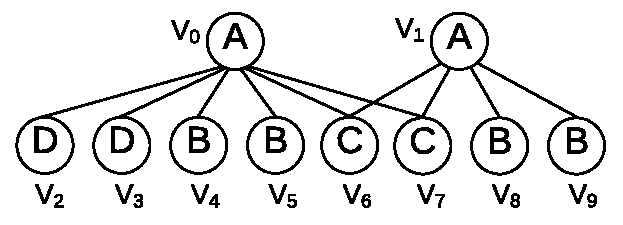
\includegraphics[scale=0.5]{img_ex/G.pdf}\hspace*{2.5em}
		\caption{data graph $G$}
		\label{fig:exactG}
	\end{subfigure}%

    \begin{subfigure}[b]{0.15\textwidth}
            % \centering
            \hspace{4mm}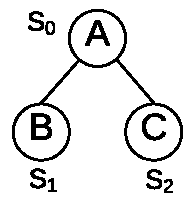
\includegraphics[scale=0.5]{img_ex/patternQ.pdf}
            \caption{Parent $Q$}
			\label{fig:exact-Q}
    \end{subfigure}%
    \hspace*{\fill}
    % \captionsetup[subfigure]{labelfont=bf,textfont=normalfont,singlelinecheck=on,justification=raggedright, skip=-5pt}
	\begin{subfigure}[b]{0.3\textwidth}
            % \centering
            \hspace{-2.5mm}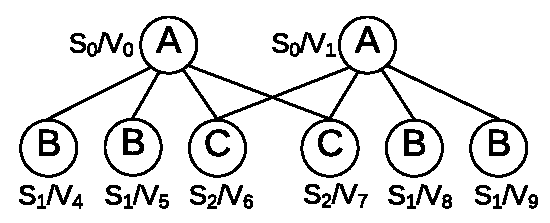
\includegraphics[scale=0.5]{img_ex/replicaQ.pdf}
            \caption{$\mathcal{R}$eplica$(Q)$}
			\label{fig:exact-REPQ}
	\end{subfigure}

	% \captionsetup[subfigure]{skip=-2pt}
	\begin{subfigure}[b]{0.15\textwidth}
		% \centering
		\hspace{4mm}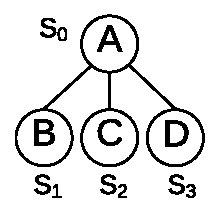
\includegraphics[scale=0.5]{img_ex/patternR.pdf}
		\caption{Child $R$}
		\label{fig:exact-R}
	\end{subfigure}%
	\hspace*{\fill}
	\begin{subfigure}[b]{0.3\textwidth}
		% \centering
		\hspace{0mm}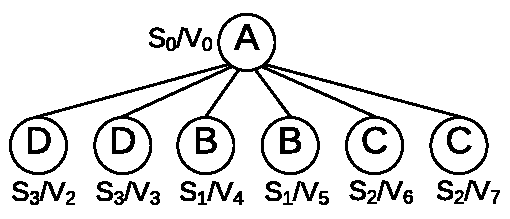
\includegraphics[scale=0.5]{img_ex/replicaR.pdf}
		\vspace{-0.25mm}
		% \vspace{-1.3\baselineskip} %not needed because figures are aligned
		% naturally unline above case
		\caption{$\mathcal{R}$eplica$(R)$}
		\label{fig:exact-REPR}
	\end{subfigure}
	% \captionsetup[figure]{skip=200pt}
    % \vspace{-1.75\baselineskip}
	\caption{$\mathcal{R}$eplica generation for a new subgraph pattern}
	\label{fig:exact-EX}
	% \vspace{0.15\baselineskip}
\end{figure}
%
%
\begin{exple}
Initially, $Q$ and $\mathcal{R}$eplica$(Q)$ are shown in Figs. \ref{fig:exact-Q}
and \ref{fig:exact-REPQ}, respectively. Child $R$, extended from $Q$ at
\emph{extending node} $s_0$ using the \emph{extending edge} $(s_0, s_3)$ is
given in Figure \ref{fig:exact-R}. Assume \emph{DFS List} for \emph{DFS}
starting at $s_0$ records edges $(s_0, s_1)$ and $(s_0, s_2)$ in that order. To
construct $\mathcal{R}$eplica$(R)$, the algorithm iterates over
$Mapping(s_0,\mathcal{R}$eplica$(Q))$, i.e. set $\{v_0, v_1\}$. With $s_0\mapsto
v_0$, the algorithm then considers vertices in $G$ (Fig. \ref{fig:exactG}) for
matching $s_3$. Thus, for each of $s_3\mapsto \{v_2, v_3\}$, the algorithm makes
recursive invocations to map $s_1$ and $s_2$ following the \emph{DFS List}
thus successfully enumerating instances. With $s_0\mapsto v_1$ however, no
mappings for matching $s_3$ exist. Graph union of all instances of $R$ thus
enumerated results in $\mathcal{R}$eplica$(R)$ depicted in Fig. \ref{fig:exact-REPR}.
% Assume, $(V_0, V_6), (V_0, V_7)\in E(G)$ map to $(A, D)$; but no such
% mapping edges exist incident to $V_1$ in $G$. All instances of $R$ thus found
% would result in $\mathcal{R}$eplica$(R)$ depicted in Figure \ref{fig:exactrepr}.
%
\end{exple}